\section{Method}
\label{section:method}

% Method: "a tool"

% Methodology: how that tool is used

% Hardware and Software used
During the experimentation, the BeagleBone Green microcontroller, Grove EMG detector, and nRF52840 Dongle were used to sample the surface EMG signals from intact limb subjects. The sampled signal was then processed to remove potential noise and artifacts from the signal. The signal is then segmented into windows. Feature extraction is then performed on each window and an investigation of dimension reduction then follows. Lastly, classification or training of the classifier is done. 

All software was written in the programming languages C and python3 version 3.10.6 64-bit. Software that was executed on the nRF52840 Dongle was written in C for the sampling of the EMG signals. Software written for the BeagleBone Green and code for offline training of the classifier was written in python3.

All code developed during this project can be found on GitHub\footnote{https://github.com/EMG4/emg\_processing} and is open source.

\begin{comment}
    To read and write to the GPIO pins on the board, the \textit{libpruio} library for C was used\footnote{https://github.com/DTJF/libpruio}.
\end{comment}
 

\subsection{Experimental setup}
The EMG sensor is placed on the wrist near the hand, see Figure~\ref{fig:elec_placement}. This placement was recommended to be used by Martin Ektröm and Daniel Morberg which were two of the instructors for the project. See Introduction~\ref{section:intro} and Botros \textit{et al}~\cite{botrosElectromyographyBasedGestureRecognition2022} for further basis on the chosen wrist placement. Before attaching the electrodes any hair is removed, the skin is cleaned with alcohol, and conductive gel is pre-applied to the electrodes to improve signal quality~\cite{khanSelectionFeaturesClassifiers2020}. The subject is seated and has their right arm resting on their leg comfortably to minimize movement and to have a fixed limb position. The subject has their right hand resting, palm facing upwards to have a fixed limb orientation. A resting position and 10 movements were performed by the subject, the movements are summarized in Table~\ref{tab:finger_movements}. These movements combined make up the total of 11 classes that are used for classification, where the class representing the resting state indicates that all fingers are open, see Figure~\ref{fig:elec_placement}. The subject is instructed to try to perform the movements using a similar amount of muscle contraction effort. When placing the electrodes, the reference electrode (black) is placed on the right lower leg. The right channel electrode (red) is placed on the left side of the wrist and the left channel electrode (white) is placed on the right side of the wrist. Description of the placement of electrodes assumes the subject's point-of-view, use of the right arm, and the palm facing upwards.

\begin{table}[ht]
    \centering
    \begin{tabular}{c|c}
        Flexion                     & Extension                        \\ \hline
        Little finger flexion(1)    & Little finger hyperextension(6)       \\
        Ring finger flexion(2)      & Ring finger hyperextension(7)         \\
        Middle finger flexion(3)    & Middle finger hyperextension(8)       \\
        Index finger flexion(4)     & Index finger hyperextension(9)        \\
        Thumb flexion(5)            & Thumb hyperextension(10)                     
    \end{tabular}
    \caption{All ten finger movements performed by the subject and their respective class, excluding the resting position (class 0).}
    \label{tab:finger_movements}
\end{table}
 
% Picture with the reference node
\begin{figure}[ht]
    \centering
    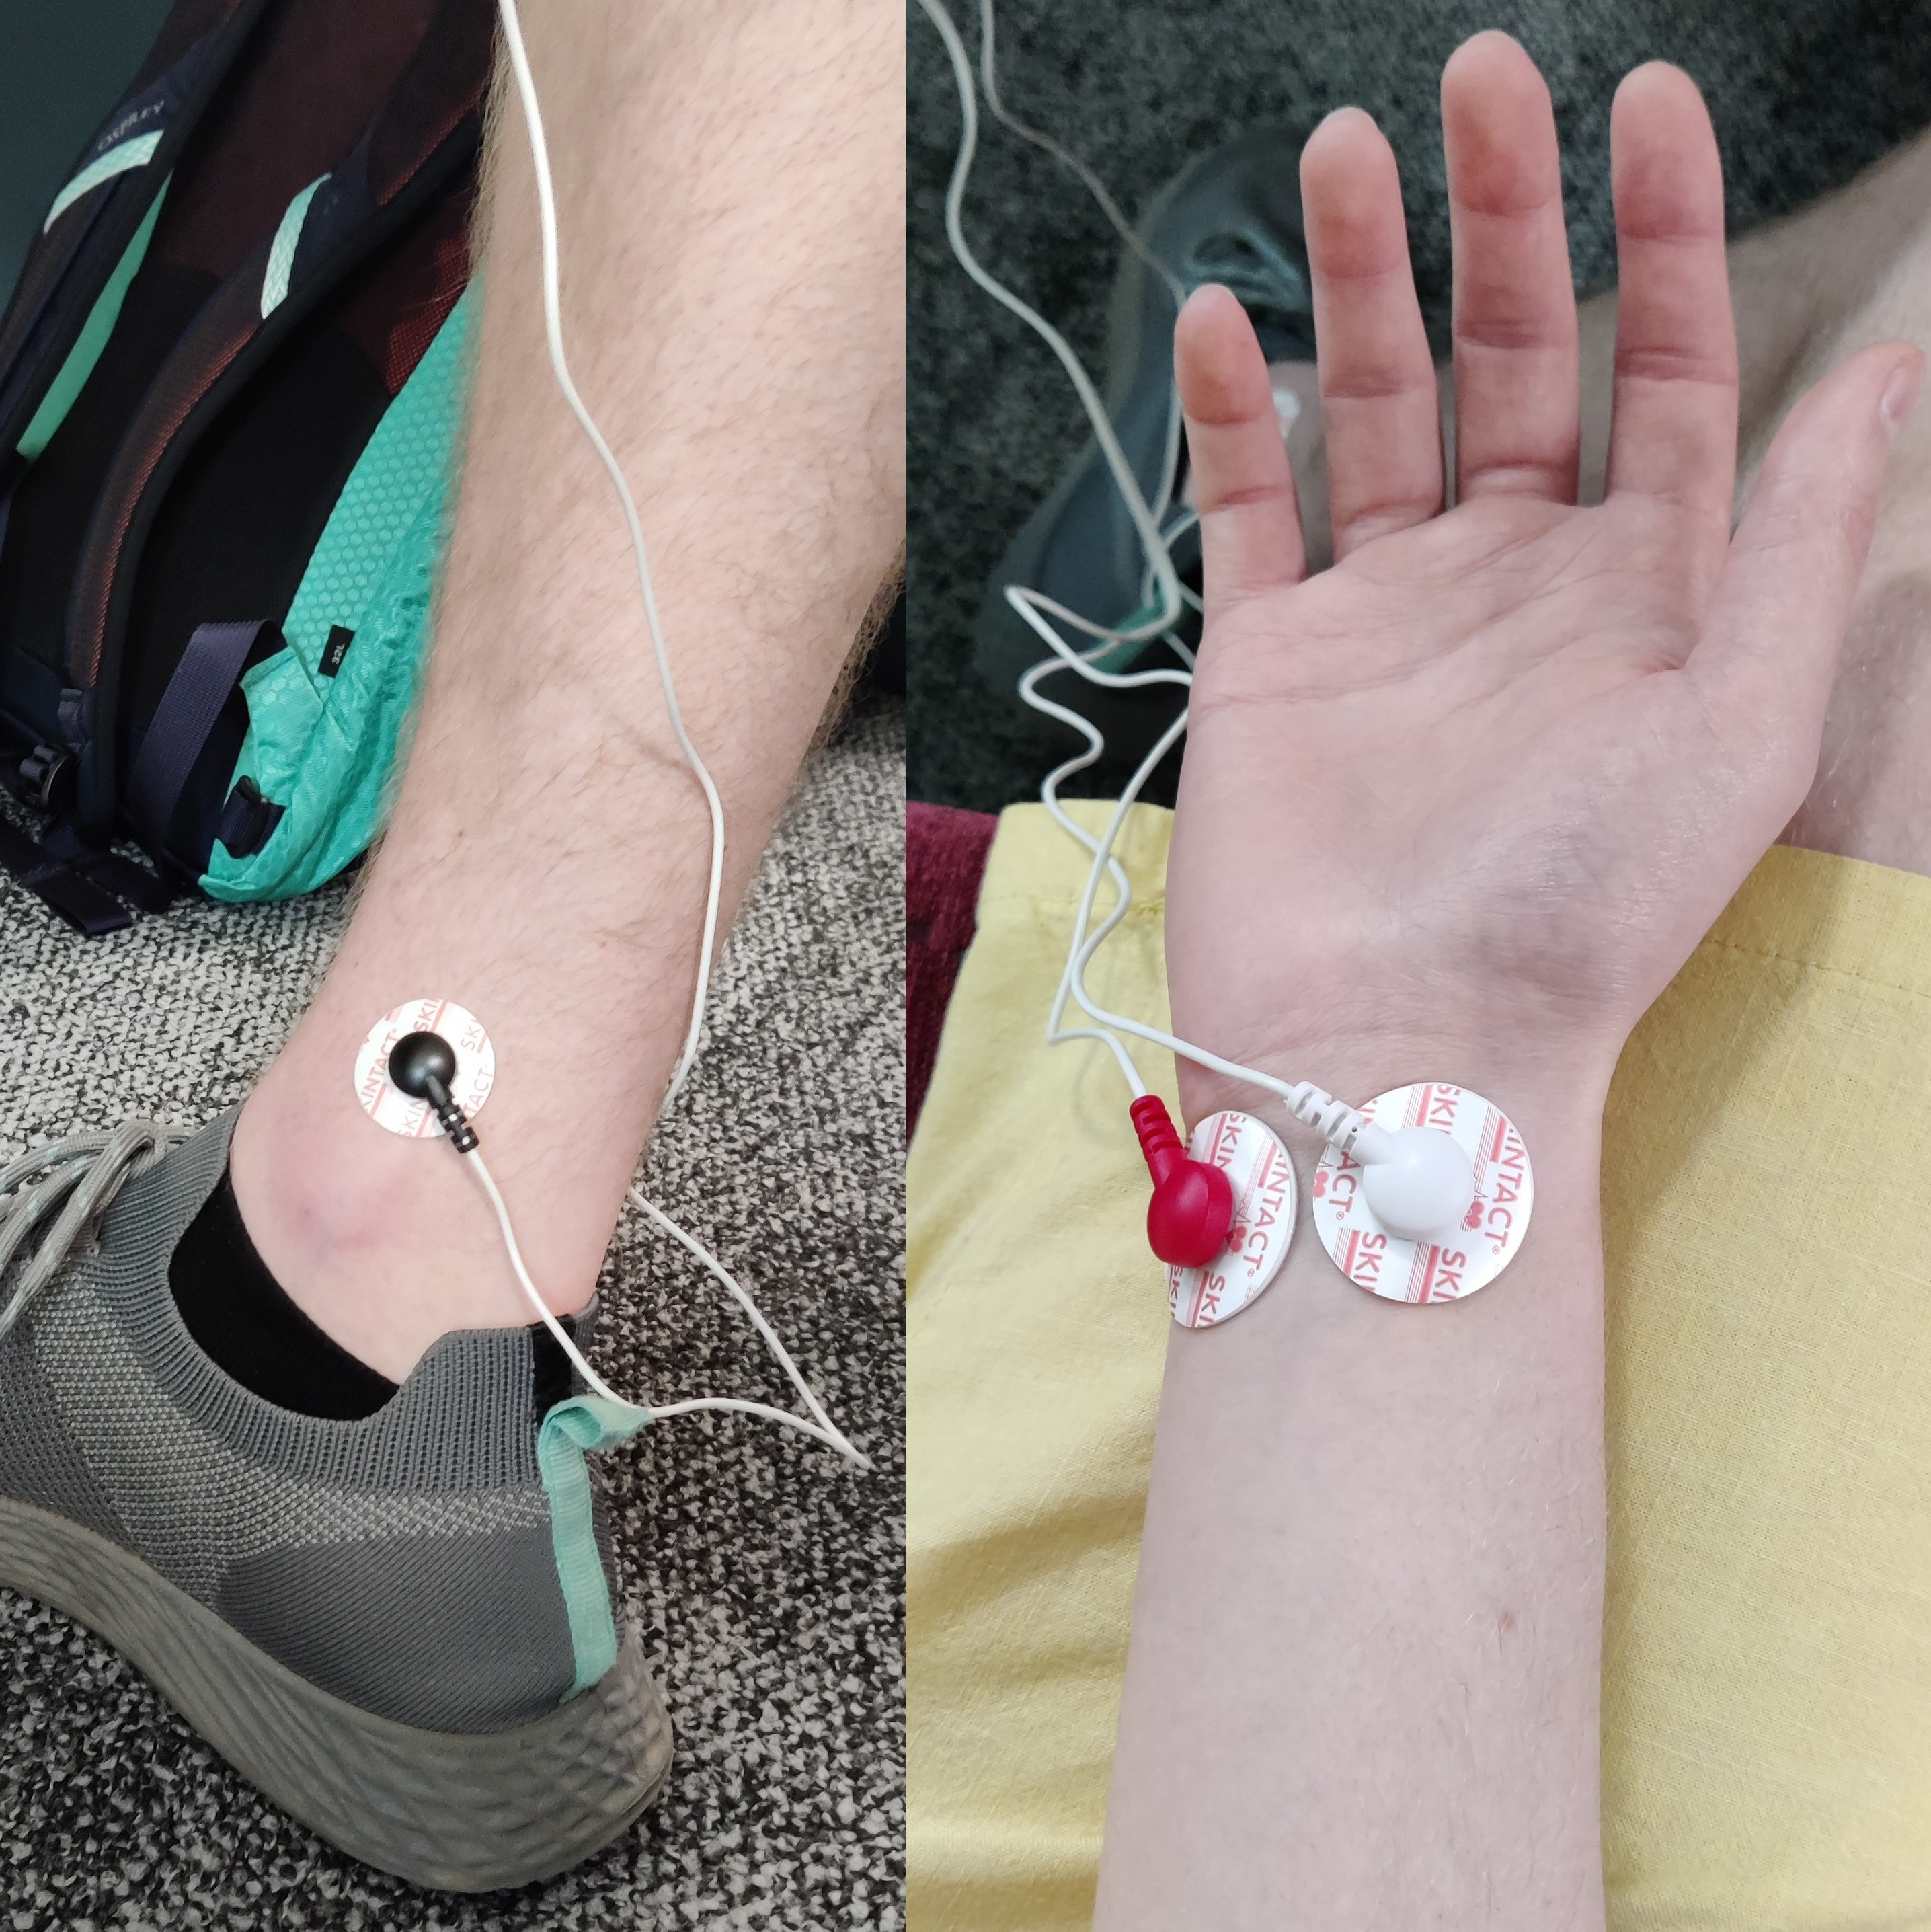
\includegraphics[width=0.9\columnwidth]{images/hand_and_reference_electrode.jpg}
    \caption{Placement of the three electrodes. The reference electrode was placed on the lower leg, the mid and end electrode were placed on the wrist.}
    \label{fig:elec_placement}
\end{figure}

% 1: Berätta om dongle
% 2: Bräda
% 3: Se till att skilja på träning och real-time classification
\subsection{Data acquisition}
The surface EMG signal was sampled using the nRF52840 Dongle as an external ADC connected to the BeagleBone Green microcontroller with a sampling frequency of 1000 Hz and using the EMG sensor Grove EMG detector. The BeagleBone Green has an input voltage range from 0 to 1.8V for its analog input and the Grove EMG detector has an output voltage range of 0 to 3.3V. Therefore the nRF52840 Dongle was used as an external ADC for sampling the Grove EMG detector voltage and sent via emulated UART over USB to the BeagleBone Green. The nRF52840 Dongle was able to sample up to 10 kHz but due to limitations of the BeagleBone Green hardware, a sampling rate of 1000 Hz was used. For training, the BeagleBone Green sent the sampled data to a laptop computer, which was used to label the data by using the laptop keyboard, via UDP. The instructor pressed a specific keyboard key depending on the movement performed by the subject. The program labeled the signal with the most recently pushed key meaning it labeled the raw data with the movement performed by the subject during run-time. The subjects performed the same movement 20 times and followed a predefined schedule. The schedule consisted of performing each movement, in numerical order according to Table~\ref{tab:finger_movements}, 5 times and then looping over from movement number 10 back to movement number 1. Each movement was maintained for 2-3 seconds. There was a resting phase of 1-2 seconds between movements. A data set was then created that consisted of EMG signals from the three authors of this paper. The data set contained a total of 60 repetitions of each movement and had a total of 5,002,128 samples. The data set contained all 11 classes, see Table \ref{tab:finger_movements}. The train test split was 0.8/0.2 because k-fold cross validation was used for evaluation with $k=5$, see Table \ref{tab:classifier_parameters}.

During live classification, data was sampled for 375 milliseconds, or 377 samples, and then forwarded to the proceeding steps of processing and classification. All functionality regarding labeling and UDP was removed from the system during this step.



\subsection{Signal processing}
% Filtering
To remove noise, a fourth-order 20 to 450 Hz bandpass filter was applied to the EMG signal, as well as a 50 Hz IIR notch filter with a quality factor of 30.
The bandpass filter was implemented using the python library pyemgpipeline version 1.0.0~\cite{PyEMGPipelinePythonPackage2022}. The notch filter was implemented using the Scipy python library version 1.10.1~\cite{2020SciPy-NMeth}.
%Removal of DC offset was done using the library pyemgpipeline version 1.0.0 \cite{PyEMGPipelinePythonPackage2022}.
% Segmentation and window
Segmentation was done using overlapping windows with a window size of 250 ms and 125 ms overlap. The window size of 250 ms and 125 ms overlap was chosen because of real-time constraints, see Introduction~\ref{section:intro}, Hristov \textit{et al}~\cite{hristovClassificationIndividualCombined2022}. 
Segmentation was implemented using the library pyemgpipeline version 1.0.0~\cite{PyEMGPipelinePythonPackage2022}. 
% Labeling
Each segment was given the label of the majority class of the samples in that segment.



\subsection{Feature extraction}
The Time Series Feature Extraction Library (TSFEL) version 0.1.5~\cite{barandas2020tsfel} was used to implement feature extraction. All features investigated were the ones available in TSFEL and can be found in the TSFEL documentation~\cite{barandas2020tsfel}. 

\begin{comment}
    Cepstral coefficients & CC \\
    Difference absolute standard deviation value & DASDV \\
    Integrated absolute value & IAV \\
    L-scale & LS \\
    Maximum fractal length & MFL \\
    Mean absolute value & MAV \\
    Mean value of the square root & MSR \\
    Root mean square & RMS \\
    Sample entropy & SampEn \\
    Time domain-auto regression & TD-AR \\
    Variance & VAR \\
    Waveform length & WL \\
    Wilson amplitude & WAMP \\
    Zero crossing & ZC
\end{comment}


\subsection{Dimensionality reduction}
The performance effect of using PCA and using no dimensionality reduction was examined.
PCA was implemented using the library scikit learn version 1.2.2~\cite{scikit-learn}.

\subsection{Classification}
Six different classifiers were investigated: ANN with GA optimization, KNN, LDA, MLP, SVM, and XGBoost. These classifiers were chosen because of their good performance in other studies (see Introduction \ref{section:intro}) and because libraries were available for these algorithms (see Introduction \ref{section:intro}). The final parameters used for these classifiers can be seen in Table \ref{tab:classifier_parameters}. The parameters in Table \ref{tab:classifier_parameters} were found through experimentation and only include parameters that were not set to the default value.
The scikit learn library version 1.2.2~\cite{scikit-learn} was used to implement KNN, LDA, MLP, and SVM. 
%The trained SVM model was too large to load on the BeagleBone Green and could thus not be tested in real-time on a microcontroller.
TensorFlow~\cite{tensorflow2015-whitepaper} Keras~\cite{chollet2015keras} version 2.12.0 was used to implement the ANN and the GA optimizer was implemented using PyGAD version 3.0.1~\cite{gadPyGADIntuitiveGenetic2021}. Note that TensorFlow could not be installed on the BeagleBone Green and thus could not be tested with live data. %\footnote{https://pygad.readthedocs.io/en/latest/index.html}. 
XGBoost was implemented using the XGBoost library version 1.7.5~\cite{Chen:2016:XST:2939672.2939785}. This library only supports 64-bit and thus could not be tested with live data because of the BeagleBone Green architecture. %\footnote{https://xgboost.readthedocs.io/en/stable/index.html}.
% Class imbalance
To prevent classifier bias, it was ensured that the training data contained the same number of entries for all classes. This was achieved by employing random over-sampling on the training data, using the library Imbalanced-learn (imblearn) version 0.10.1~\cite{JMLR:v18:16-365}.

\begin{table}[ht]
    \centering
    \begin{tabular}{c|c|c}
        Algorithms & Parameter & Value \\ \hline
        All & K-fold & 5 \\
        ANN & Dropout Rate & 0.1 \\
        ANN & Layers & 3 \\
        ANN & Neurons & 5 \\
        ANN, MLP & Solver function & adam \\
        ANN, MLP & Activation function & relu \\
        ANN. MLP & Max number of iterations & 10000 \\
        ANN & Batch size & 10 \\
        ANN & Number of classes & 11 \\
        GA & Number of solutions in population & 100 \\
        GA & Number of number of generations & 200 \\
        GA & Number of parents mating & 40 \\
        KNN & Number of neighbors & 2 \\
        KNN & Number of leafs & 10 \\
        KNN & Weight function & distance \\
        LDA & LDA solver & eigen \\
        MLP & Layers & 7 \\
        MLP & Learning rate model & constant \\
        MLP & Learning rate ($\alpha$) & 0.01 \\
        SVM & Kernel & rbf \\
        SVM & Gamma & auto \\
        SVM & Decision function shape & ovr                      
    \end{tabular}
    \caption{Classifier parameters used that was not set to the default value.}
    \label{tab:classifier_parameters}
\end{table}

The library SkLearn2PMML version 0.92.2~\cite{ruusmannSkLearn2PMML2023}
%\footnote{https://github.com/jpmml/sklearn2pmml} 
was used for saving the trained classifier to a PMML file. The trained classifier was then loaded onto the BeagleBone Green from the PMML file using the library JPMML-Evaluator-Python version 0.10.0~\cite{ruusmannJPMMLEvaluatorPython2023}. %\footnote{https://github.com/jpmml/jpmml-evaluator-python}. 
Both of these libraries are part of the Java PMML API~\cite{ruusmannJavaPMMLAPI2023}.
%\footnote{https://github.com/jpmml}. 
The BeagleBone Green has a 32-bit ARMV7 architecture which is the cause for using PMML. When using python3, Pickle and other similar methods should be avoided for the deployment of the model on a different system unless all systems use the same version of software and run the same bit architecture\footnote{https://github.com/scikit-learn/scikit-learn/issues/19602}.



% In this section, the method used to find an answer to the research questions should be presented. 

% If this report presents results from a literature search, this means providing sufficient information for allowing someone else to repeat the literature search and compare the results. I.e., a search using the phrases a, b, and c, was made in database x, y and z on the date Month Date, Year (e.g., July 31st, 2021). The search resulted in x hits. Then, information on how you chose which works to include in this report should be provided. The references should be used for answering your research questions.

% If the work reports on an experiment, this part should provide information about the experimental setup, how the experiment was conducted, how data was collected and analyzed etc. Motivate methodological choices through references. Also an experiment should be presented with sufficient detail such that it can be repeated by someone else.